\subsection{Architectural Patterns}
\subsubsection{Model-View-Controller}
We will use the MVC pattern to implement the user interface.
\begin{itemize}
	\item{Model}
	\newline
	The model will be implemented by making use of Express.js
	\item{View}
	\newline
	The view will be implemented using Angular Material, initially Bootstrap was going to be used.
	\item{Controller}
	\newline
	The controller will be implemented by using Angular.js
	\begin{figure}[H]
	    	\centering
	    	\fbox{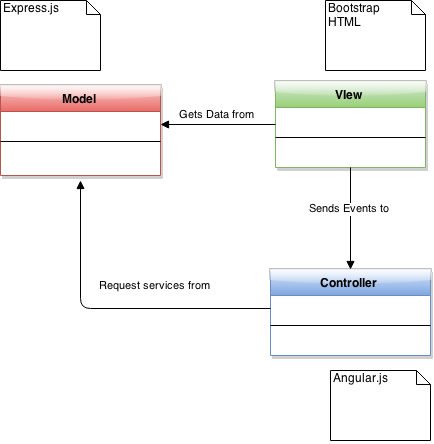
\includegraphics[width=0.5\textwidth]{MVC}}
	    	\caption{Model View Controller}
	    	\label{fig:Learning rate 0.1}
   	\end{figure}
	The purpose of the MVC is to decouple the entities from each other. This will allow us to build Phonegap apps out of our client side. Each component can then evolve on its own through the development phase. 
	The properties of the MVC that we want to take advantage of is as follows:
	\begin{itemize}
		\item Simplification through separation of concerns.
		\item Reuse of the view components.
		\item Maintainability, that facilitates the development by different team members.
		\item Testability as testing is a crucial part of our design and thus this has great influence.
	\end{itemize}
\end{itemize}

\subsubsection{Observer Design Pattern}
The mediator pattern is used by the Socket.IO library to allow real-time updating of a page during estimation. The main purpose is to ensure that estimators are able to communicate with each other in real-time by commenting on specific nodes and discussing possible confusion or ambiguity and also avoid race conditions when many estimators are attempting to change the project tree at the same time. When an estimator comments on a project feature or edits the project tree the server is notified of the change and it then propagates the new updated project state to all of the remote users currently viewing the project tree or discussion thread.
\begin{itemize}
	\item{Observers}
	\newline
	The client-side users will notify the subject of local changes.
	\item{Subject}
	\newline
	The server will act as the subject and notify any connected users of the updated state of the discussion or project.
\end{itemize}